\documentclass[10pt,landscape]{article}
\usepackage{multicol}
\usepackage{calc}
\usepackage{ifthen}
\usepackage[landscape]{geometry}
\usepackage{listings}
\usepackage{amsmath,amsthm,amsfonts,amssymb}
\usepackage{mathtools}
\usepackage{color,graphicx,overpic}
\usepackage{hyperref}
\usepackage[dvipsnames]{xcolor}

\usepackage{MnSymbol}
\usepackage{graphicx}
\usepackage{wrapfig}
\usepackage{tikz}

\usepackage{blindtext}

% This sets page margins to .1 inch if using letter paper, and to 1cm
% if using A4 paper. (This probably isn't strictly necessary.)
% If using another size paper, use default 1cm margins.
\ifthenelse{\lengthtest { \paperwidth = 11in}}
    { \geometry{top=0.2in,left=0.2in,right=0.2in,bottom=0.2in} }
    {\ifthenelse{ \lengthtest{ \paperwidth = 297mm}}
        {\geometry{top=1cm,left=1cm,right=1cm,bottom=1cm} }
        {\geometry{top=1cm,left=1cm,right=1cm,bottom=1cm} }
    }

% Turn off header and footer
\pagestyle{empty}

% Redefine section commands to use less space
\makeatletter
\renewcommand{\section}{\@startsection{section}{1}{0mm}%
                                {-1ex plus -.5ex minus -.2ex}%
                                {0.5ex plus .2ex}%x
                                {\normalfont\large\bfseries}}
\renewcommand{\subsection}{\@startsection{subsection}{2}{0mm}%
                                {-1ex plus -.5ex minus -.2ex}%
                                {0.5ex plus .2ex}%
                                {\normalfont\normalsize\bfseries}}
\renewcommand{\subsubsection}{\@startsection{subsubsection}{3}{0mm}%
                                {-1ex plus -.5ex minus -.2ex}%
                                {0.5ex plus .2ex}%
                                {\normalfont\footnotesize\bfseries}}
\makeatother

% Itemize to use less space
\usepackage{enumitem}
\setlist{leftmargin=*, nosep}
\setenumerate{nosep}

% Define BibTeX command
\def\BibTeX{{\rm B\kern-.05em{\sc i\kern-.025em b}\kern-.08em
    T\kern-.1667em\lower.7ex\hbox{E}\kern-.125emX}}

% Don't print section numbers
\setcounter{secnumdepth}{0}


\setlength{\parindent}{0pt}
\setlength{\parskip}{0pt plus 0.5ex}

%My Environments
\newtheorem{example}[section]{Example}

\newcommand{\Blue}[1]{\noindent{\textcolor{Blue}{\textbf{#1}}}:}
\newcommand{\Red}[1]{\noindent{\textcolor{BrickRed}{\textbf{#1}}}:}
\newcommand{\Green}[1]{\noindent{\textcolor{PineGreen}{\textbf{#1}}}:}
\newcommand{\Hint}[1]{\noindent{\textcolor{Orange}{#1}}}

\newcommand*{\eg}{e.g.\@\xspace}
\newcommand*{\ie}{i.e.\@\xspace}
\newcommand*{\Eg}{E.g.\@\xspace}
\newcommand*{\Ie}{I.e.\@\xspace}
\newcommand*{\esp}{esp.\@\xspace}
\newcommand*{\wrt}{\ifmmode \stext{w.r.t.} \else w.r.t.\@\xspace \fi}


\usepackage{draftwatermark}
% Configure the watermark
\SetWatermarkText{Made with love by \texttt{junruren}} % Set the watermark text
\SetWatermarkScale{2}            % Adjust the scale of the watermark
\SetWatermarkLightness{0.97}      % Set the lightness (closer to 1 is more faded)
% -----------------------------------------------------------------------

\begin{document}
\raggedright
\scriptsize

\begin{multicols}{4}
% multicol parameters
% These lengths are set only within the two main columns
%\setlength{\columnseprule}{0.25pt}
\setlength{\premulticols}{1pt}
\setlength{\postmulticols}{1pt}
\setlength{\multicolsep}{1pt}
\setlength{\columnsep}{2pt}

\subsection{H1 (selected)}

\Red{Elasticity} meansure of price sensitivity
\Blue{Own-price elasticity of demand $\frac{\% \Delta Q_1^D}{\% \Delta P_1}$} the \% change in quantity demanded for a
1\% change in its price. Always negative by Law of Demand. $|E| \begin{cases}
    < 1 & \text{Inelastic} \\
    > 1 & \text{Elastic}
\end{cases}$

\Blue{Cross-price elasticity of demand $\frac{\% \Delta Q_1^D}{\% \Delta P_2}$} the \% change in quantity demanded for a
1\% change in \underline{another good's} price. $\begin{cases}
    > 0 & \text{SUBSTITUTES (wine \& beer)} \\
    < 0 & \text{COMPLEMENTS (popcorn \& beer)}
\end{cases}$

\Red{Network Externality} The product is more valuable to you if it is used by others. To maintain n.e., (1) establish
switching costs (2) interoperability (weakens direct n.e.)
\begin{itemize}
    \item Direct n.e.: Emails -- requires other users
    \item Indirect n.e.: Windows -- requires complements like software developed for Win.
\end{itemize}
\Blue{Positive N.E.} the value of a product increases with the \# of users (higher WTP). Network goods. Makes demand \textit{more
elastic} so an aggressive pricing strategy becomes more profitable.
\Blue{Negative N.E.} e.g. luxury goods.

\Red{Monopoly} a single firm is in the market.

\Blue{Marginal Cost (MC)} How cost changes as output $Q$ changes: for 1 unit, $Cost(Q) - Cost(Q-1)$ ; for more units,
$\frac{\Delta Cost}{\Delta Q}$; and for small changes, $\frac{d Cost}{d Q}$. \Hint{Fixed costs don't enter MC.}

\Blue{Marginal Revenue (MR)} in order to sell more units, the price must be lowered for all units.
\fbox{$MR = \frac{\Delta Rev(Q)}{\Delta Q} = P(Q) + Q \frac{\Delta P(Q)}{\Delta Q}$}

\begin{multicols}{2}

Decrease price results in: \textbf{\textcolor{Green}{gain}} in Rev from Q increases + \textbf{\textcolor{Red}{loss}} in Revenue from P reduction for all units.

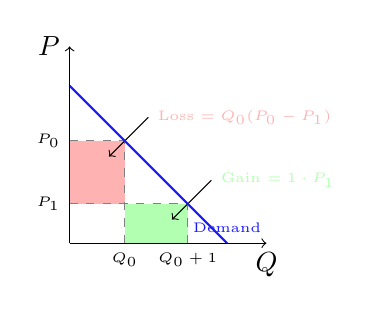
\begin{tikzpicture}
    % Loss
    \fill[red!30] (0, 1.3) -- (0.7, 1.3) -- (0.7, 0.5) -- (0, 0.5) -- cycle;
    \draw[<-] (0.5, 1.1) -- (1, 1.6) node[right,red!30] {\tiny Loss $=Q_0 (P_0 - P_1)$};
    % Gain
    \fill[green!30] (0.7, 0) -- (0.7, 0.5) -- (1.5, 0.5) -- (1.5, 0) -- cycle;
    \draw[<-] (1.3, 0.3) -- (1.8, 0.8) node[right,green!30] {\tiny Gain $= 1 \cdot P_1$};

    \draw[dashed,gray] (0, 1.3) -- (0.7, 1.3);
    \draw[dashed,gray] (0.7, 0) -- (0.7, 1.3);
    \draw[dashed,gray] (0, 0.5) -- (1.5, 0.5);
    \draw[dashed,gray] (1.5, 0) -- (1.5, 0.5);
    \draw[thick,blue!90] (0,2) -- (2,0) node[above] {\tiny Demand}; % D
    % Draw axes
    \draw[->] (0,0) -- (2.5,0) node[anchor=north] {$Q$};
    \draw[->] (0,0) -- (0,2.5) node[anchor=east] {$P$};
    
    % Label values
    \node[anchor=north] at (0.7,0) {\tiny $Q_0$};
    \node[anchor=east] at (0,1.3) {\tiny $P_0$};
    \node[anchor=north] at (1.5,0) {\tiny $Q_0 + 1$};
    \node[anchor=east] at (0,0.5) {\tiny $P_1$};

\end{tikzpicture}
\end{multicols}

If demand curve linear, \Hint{MR has same intercept and twice the slope. $P(Q) = 100 - Q \rightarrow MR = 100 - 2 Q$}

\begin{multicols}{2}
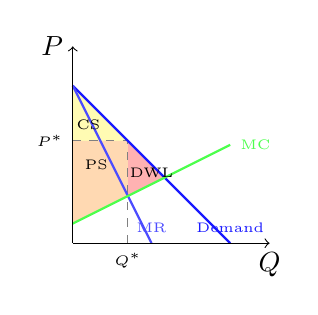
\begin{tikzpicture}
    % CS
    \fill[yellow!30] (0, 1.3) -- (0.7, 1.3) -- (0, 2) -- cycle;

    %DWL
    \fill[red!30] (0.7, 0.6) -- (0.7, 1.3) -- (1.167, 0.833) -- cycle;

    %PS
    \fill[orange!30] (0, 0.25) -- (0, 1.3) -- (0.7, 1.3) -- (0.7, 0.6) -- cycle;

    \draw[dashed,gray] (0, 1.3) -- (0.7, 1.3);
    \draw[dashed,gray] (0.7, 0) -- (0.7, 1.3);
    \draw[thick,blue!90] (0,2) -- (2,0) node[anchor=south] {\tiny Demand}; % D
    \draw[thick, blue!70] (0,2) -- (1,0) node[anchor=south] {\tiny MR}; % MR
    \draw[thick, green!70] (0,0.25) -- (2,1.25) node[anchor=west] {\tiny MC}; % MC
    % Draw axes
    \draw[->] (0,0) -- (2.5,0) node[anchor=north] {$Q$};
    \draw[->] (0,0) -- (0,2.5) node[anchor=east] {$P$};
    
    % Label values
    \node[anchor=north] at (0.7,0) {\tiny $Q^*$};
    \node[anchor=east] at (0,1.3) {\tiny $P^*$};
    \node at (0.2,1.5) {\tiny CS};
    \node at (0.3,1) {\tiny PS};
    \node at (1,0.9) {\tiny DWL};

\end{tikzpicture}

\Green{Profix Maximization} optimal $Q^*$ when $MC(Q^*) = MR(Q^*)$. Then solve for optimal price $P^* =P(Q^*)$
\Hint{Does not depend on the level of demand.}

\Green{Mark-up Formula} resulting from profit-max, $P^*$ satisfies: $\frac{P-MC}{P} = -\frac{1}{\epsilon}$ ($\epsilon$ is the demand elasticity).
\Hint{Relatively more elastic markets (markets with more price-sensitive consumers) will face smaller markups} (i.e., lower prices if costs are the same across markets).
\end{multicols}

\subsection{H2}
\subsubsection{Supply and Demand}

\Red{Demand} how much consumers will buy at a particular price; describes consumers' willingness to pay (WTP).
\fbox{$Q_d = a - b \cdot P$}

\Red{Supply} how much producers will provide at a particular price; describes producers' willingness to accept (WTA) /
the industry's aggregate marginal cost curve (\ie Market supply is the \underline{sum} of the
individual firm supply curves).
\fbox{$Q_s = c + d \cdot P$}

\Hint{\underline{Remember} to always check whether we need to \underline{invert} a given function!}
\Blue{Competitive Markets} Individual firms and consumers don't affect prices (\ie they have no market power and are
price takers)

\Red{Competitive Market Equilibrium} \fbox{$Q^* = Q_s (P^*) = Q_d (P^*)$}
In these markets, \Hint{prices are determined} by:
\begin{itemize}
    \item the \Blue{``marginal buyer'' $P^* = WTP$} who would leave the market if the price were any higher, and
    \item the \Blue{``marginal seller'' $P^* = WTA$} who would leave the market if the price were any lower
\end{itemize}

\Blue{Producer Surplus (PS)} = Revenue - Total WTA = Revenue - Total Variable Cost (area below price and above supply.)

Without market power, \Hint{firm-level inverse demand curve is perfectly elastic} (\ie horizontal) \Hint{at the market
price.} Market sets \fbox{$MR(Q) = P$}. \Hint{Firm's supply curve is its MC curve}. Firm profit \textbf{maximized} when:
\fbox{$\text{Market } P = MR(Q^*) = MC(Q^*)$}, provided the firm is operating at all.
\textit{Not to be confused with
the MR discussed in H1 Monopoly Pricing!}

\Red{First Welfare Theorem} Competitive markets are \textbf{efficient} (\ie they maximize total surplus = CS + PS).
\begin{itemize}
    \item Assumes no distortions such as market power, info frictions, or \textit{externalities}.
    \item Under perfect competition, all trades involving consumers who value the good more than the marginal cost associated with producing an additional unit of the good are realized.
\end{itemize}

\Blue{Welfare is maximized} by the perfectly competitive outcome when there are not externalities.
To maximize total welfare, we want
\begin{itemize}
    \item Consumers get: $CS = \frac{1}{2} (a - P^*)Q^*$
    \item Producers get: $PS = \frac{1}{2} (P^* - c)Q^*$
\end{itemize}

\begin{multicols}{2}
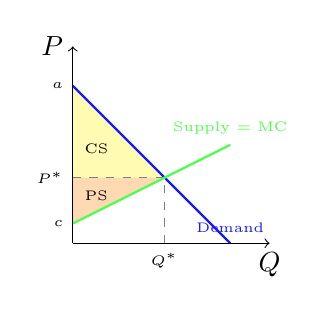
\begin{tikzpicture}
    % CS
    \fill[yellow!30] (0, 0.83) -- (1.16, 0.83) -- (0, 2) -- cycle;

    %PS
    \fill[orange!30] (0, 0.25) -- (0, 0.83) -- (1.16, 0.83) -- cycle;

    \draw[dashed,gray] (0, 0.83) -- (1.16, 0.83);
    \draw[dashed,gray] (1.16, 0) -- (1.16, 0.83);
    \draw[thick,blue!90] (0,2) -- (2,0) node[anchor=south] {\tiny Demand}; % Demand curve
    \draw[thick, green!70] (0,0.25) -- (2,1.25) node[anchor=south] {\tiny Supply = MC}; % Supply curve
    % Draw axes
    \draw[->] (0,0) -- (2.5,0) node[anchor=north] {$Q$};
    \draw[->] (0,0) -- (0,2.5) node[anchor=east] {$P$};
    
    % Label values
    \node[anchor=north] at (1.16,0) {\tiny $Q^*$};
    \node[anchor=east] at (0,0.83) {\tiny $P^*$};
    \node[anchor=east] at (0,0.25) {\tiny $c$};
    \node[anchor=east] at (0,2) {\tiny $a$};
    \node at (0.3,1.2) {\tiny CS};
    \node at (0.3,0.6) {\tiny PS};

\end{tikzpicture}
Competitive markets maximize total surplus.
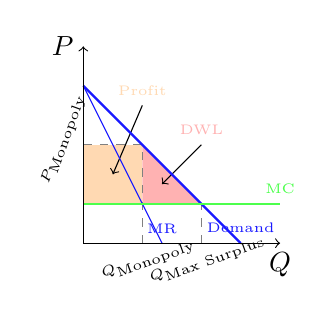
\begin{tikzpicture}
    %DWL
    \fill[red!30] (0.75, 0.5) -- (0.75, 1.25) -- (1.5, 0.5) -- cycle;
    \draw[<-] (1, 0.75) -- (1.5, 1.25) node[anchor=south,red!30] {\tiny DWL};

    %Profit
    \fill[orange!30] (0, 0.5) -- (0, 1.25) -- (0.75, 1.25) -- (0.75, 0.5) -- cycle;
    \draw[<-] (0.375, 0.875) -- (0.75, 1.75) node[anchor=south,orange!30] {\tiny Profit};

    \draw[dashed,gray] (0, 1.25)  -- (0.75, 1.25); % P_monopoly dashed line
    \draw[dashed,gray] (0.75, 0) -- (0.75, 1.25); % Q_monopoly dashed line
    \draw[dashed,gray] (1.5, 0) -- (1.5, 0.5); % Q_max surplus dashed line
    \draw[thick,blue!90] (0,2) -- (2,0) node[anchor=south] {\tiny Demand}; % Demand curve
    \draw[blue!90] (0,2) -- (1,0) node[anchor=south] {\tiny MR}; % MR curve
    \draw[thick, green!70] (0,0.5) -- (2.5,0.5) node[anchor=south] {\tiny MC}; % Supply curve
    % Draw axes
    \draw[->] (0,0) -- (2.5,0) node[anchor=north] {$Q$};
    \draw[->] (0,0) -- (0,2.5) node[anchor=east] {$P$};
    
    % Label values
    \node[anchor=north, rotate=20] at (0.75,0) {\tiny $Q_{\text{Monopoly}}$};
    \node[anchor=north, rotate=20] at (1.5,0) {\tiny $Q_{\text{Max Surplus}}$};
    \node[anchor=east, rotate=70] at (0,2) {\tiny $P_{\text{Monopoly}}$};

\end{tikzpicture}
Distortion \eg: Pricing with market power
\end{multicols}

\Red{Deadweight Loss (DWL)} Lost surplus due to a distortion away from perfect competition. \fbox{DWL = CS + PS - TS} \ie Maximum surplus - Achieved surplus. DWL offers an opportunity to ``grow the pie'', represents the value proposition for many firms.

\Green{In the left graph} DWL will be generated
\begin{itemize}
    \item if $Q < Q^*$ because there will be consumers that value the product at above the marginal cost
    \item if $Q > Q^*$ because there will be consumers consuming the product even though their $WTP < MC$
\end{itemize}

\Red{Cost Shock} if one side of the market is highly elastic, then they can avoid shocks (and pass on any taxes / transation fees).
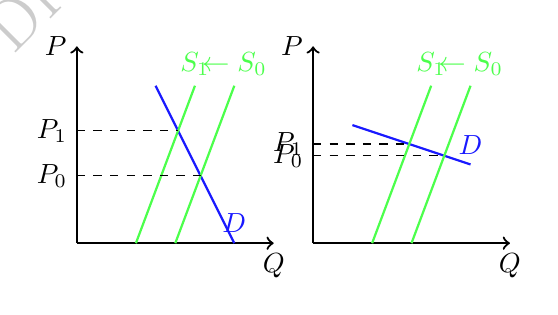
\begin{tikzpicture}

    % LEFT GRAPH
    % Axes
    \draw[thick,->] (0,0) -- (2.5,0) node[anchor=north] {$Q$};
    \draw[thick,->] (0,0) -- (0,2.5) node[anchor=east] {$P$};
    
    % Demand Curve
    \draw[thick,blue!90] (1,2) -- (2,0) node[above] {$D$};
    
    % Supply Curves
    \draw[thick,green!70] (1.25,0) -- (2,2) node[above] {$\leftarrow S_0$};
    \draw[thick,green!70] (0.75,0) -- (1.5,2) node[above] {$S_1$};
    
    % Price levels
    \draw[dashed] (0,1.4285714286) -- (1.2857142857,1.4285714286) node[left] at (0,1.4285714286) {$P_1$};
    \draw[dashed] (0,0.8571428571) -- (1.5714285714,0.8571428571) node[left] at (0,0.8571428571) {$P_0$};
    
    % RIGHT GRAPH
    \begin{scope}[shift={(3,0)}] % Shift to the right for the second plot
    % Axes
    \draw[thick,->] (0,0) -- (2.5,0) node[anchor=north] {$Q$};
    \draw[thick,->] (0,0) -- (0,2.5) node[anchor=east] {$P$};
    
    % Demand Curve
    \draw[thick,blue!90] (0.5,1.5) -- (2,1) node[above] {$D$};
    
    % Supply Curves
    \draw[thick,green!70] (1.25,0) -- (2,2) node[above] {$\leftarrow S_0$};
    \draw[thick,green!70] (0.75,0) -- (1.5,2) node[above] {$S_1$};
    
    % Price levels
    \draw[dashed] (0,1.2592592593) -- (1.2222222222,1.2592592593) node[left] at (0,1.2592592593) {$P_1$};
    \draw[dashed] (0,1.1111111111) -- (1.6666666667,1.1111111111) node[left] at (0,1.1111111111) {$P_0$};
    
    \end{scope}
\end{tikzpicture}

\subsubsection{Externalities}

\Red{Externality} an activity generates it when it imposes a cost or benefit on a third party not involved in the activity. An externality is a \textbf{market failure} because the market does not account for the full cost or benefit of the activity -- left alone the perfectly competitive market will not maximize welfare.
\begin{itemize}
    \item \Blue{Negative ext.} costs born by society; \eg pollution, congestion, noise, contagion. External costs (negative ext.) $\Rightarrow$ firms produce too much. \Green{Sol.} tax the product by the externaltiy amount (to shift \textbf{up the \underline{supply} curve}); \Hint{taxes ``internalize'' the externality and reduce quantity.}
    \item \Blue{Positive ext.} benefits born by society; \eg education, vaccines, R\&D (ideas). External benefits (positive ext.) $\Rightarrow$ firms produce too little. \Green{Sol.} subsidize \underline{customers} the externaltiy amount (to shift \textbf{up the \underline{demand curve}})
\end{itemize}
Without solutions (\eg regulation, taxes, subsidies, property rights), externalities create DWL.

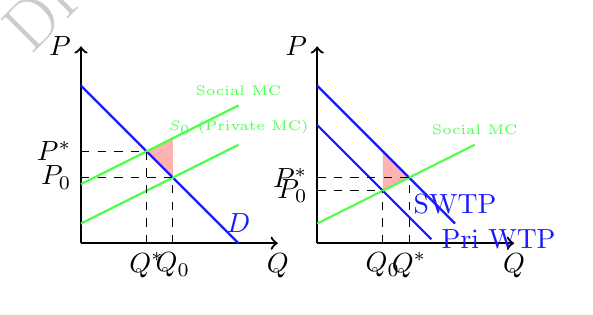
\begin{tikzpicture}
    % LEFT GRAPH
    % Axes
    \draw[thick,->] (0,0) -- (2.5,0) node[anchor=north] {$Q$};
    \draw[thick,->] (0,0) -- (0,2.5) node[anchor=east] {$P$};

    % DWL
    \fill[red!30] (1.1666666667, 0.8333333333) -- (1.1666666667, 1.3333333333) -- (0.8333333333, 1.1666666667) -- cycle;
    
    % Demand Curve
    \draw[thick,blue!90] (0,2) -- (2,0) node[above] {$D$};
    
    % Supply Curves
    \draw[thick,green!70] (0, 0.75) -- (2, 1.75) node[above] {\tiny Social MC};
    \draw[thick,green!70] (0, 0.25) -- (2,1.25) node[above] {\tiny $S_0$ (Private MC)};
    
    % Price levels
    \draw[dashed] (0,1.1666666667) -- (0.8333333333,1.1666666667) node[left] at (0,1.1666666667) {$P^*$};
    \draw[dashed] (0,0.8333333333) -- (1.1666666667,0.8333333333) node[left] at (0,0.8333333333) {$P_0$};
    \draw[dashed] (0.8333333333,0) -- (0.8333333333,1.1666666667) node[below] at (0.8333333333,0) {$Q^*$};
    \draw[dashed] (1.1666666667,0) -- (1.1666666667,0.8333333333) node[below] at (1.1666666667,0) {$Q_0$};
    
    % RIGHT GRAPH
    \begin{scope}[shift={(3,0)}] % Shift to the right for the second plot
    \draw[thick,->] (0,0) -- (2.5,0) node[anchor=north] {$Q$};
    \draw[thick,->] (0,0) -- (0,2.5) node[anchor=east] {$P$};

    % DWL
    \fill[red!30] (1.1666666667, 0.8333333333) -- (0.8333333333, 0.6666666667) -- (0.8333333333, 1.1666666667) -- cycle;
    
    % Demand Curve
    \draw[thick,blue!90] (0,2) -- (1.75,0.25) node[above] {SWTP};
    \draw[thick,blue!90] (0,1.5) -- (1.45,0.05) node[right] {Pri WTP};
    
    % Supply Curves
    \draw[thick,green!70] (0, 0.25) -- (2,1.25) node[above] {\tiny Social MC};
    
    % Price levels
    \draw[dashed] (0,0.6666666667) -- (0.8333333333,0.6666666667) node[left] at (0,0.6666666667) {$P_0$};
    \draw[dashed] (0,0.8333333333) -- (1.1666666667,0.8333333333) node[left] at (0,0.8333333333) {$P^*$};
    \draw[dashed] (0.8333333333,0) -- (0.8333333333,0.6666666667) node[below] at (0.8333333333,0) {$Q_0$};
    \draw[dashed] (1.1666666667,0) -- (1.1666666667,0.8333333333) node[below] at (1.1666666667,0) {$Q^*$};
    \end{scope}
\end{tikzpicture}

\Blue{Tragedy of the Commons} When a resource is held in common, individuals have no incentive to conserve it. This is
an example of a negative externality since others' access impairs everyone's use of the resource. Individual will
overuse. \Green{Solution} assign property rights, regulate, or tax; joint ventures also allow for collaboration that
``internalizes'' the externality.

\Blue{Coase Theorem} If property rights are well-defined and \underline{transaction costs} are low (or none), the
efficient solution occurs regardless of who holds the property rights. Cap and Trade policies set up a market to make
this bargaining easier.

\Blue{Distributional Consequences}
\begin{enumerate}
    \item the distribution of the burden of the externality,
    \item distribution of the costs to correct the externality, and
    \item distribution of the burden of externality after policy intervention.
\end{enumerate}

\Green{\Eg the R\&D market} think of the demand curve originating from the profits that firms here would get from
innovating, and thus representing the \textbf{private} demand for R\&D. The MC curve (supply) represents the private MC
of research and development. We will assume that the private MC of R\&D equals the social MC. Demand:
$Q_{\text{private},d} = 100 - 2P$; supply: $Q_s = \frac{P}{2}$.
\begin{enumerate}
    \item \Green{Competitive market equilibrium} $Q_{\text{private},d} = Q_s \Rightarrow 100-2P = \frac{P}{2} \Rightarrow \begin{cases}
        P^* = 40 \\
        Q_s^* = 20
    \end{cases}$
    \item \Green{Total amount spent on R\&D} $P^* \cdot Q_s^* = 40 \cdot 20 = 800$
    \item Now suppose that not only does the firm paying for the research and development benefit from the R\&D, but some of these benefits spillover to other firms. In particular, economists have calculated that every unit of R\&D done by a firm benefits other firms by \$30. \Green{What is the \textbf{society} demand curve for R\&D} Inverse demand curve: $P = 50 - \frac{Q}{2}$. The positive externality implies that the willingness to pay for R\&D increases by \$30 everywhere. So the social inverse demand curve (SWTP) is $P = 80 - \frac{Q}{2} \xRightarrow{\text{inverse}} Q_{\text{society},d} = 160 - 2P$
    \item \Green{Ways to overcome this positive externality} \begin{enumerate}
        \item Implementing patent system to allow the innovating firm to capture more of the benefits from their R\&D.
        \item Subsidizing R\&D; \esp for hard, basic science.
    \end{enumerate}
\end{enumerate}

\subsubsection{Game Theory}

\Hint{Each player's objective is to maximize their payoff}, not to beat their opponent.

\Red{Situation of strategic interdependence} a firm's best choice depends on what its rivals do and how it expects rivals to react to its actions.

\Blue{Strategy} a ``complete contingent plan'' that specifies what a player will do at every possible decision node.

\Blue{Best response} the strategy with the highest payoff in response to the strategies its rivals can take.

\Blue{Dominant Strategy} a strategy that is best for a player to follow regardless of the strategies chosen by other players. \Hint{It's a player's best response to any strategy the other player might choose.}

\Blue{Iterated dominance} sometimes it's possible to narrow things down by eliminating strategies that known never a best choice for rival, and also strategies that are never a best choice for rival if they eliminate the possibility that you will play something that's never a best choice for you \dots \Green{\Eg} guess half of thge median game.

\Red{Nash Equilibrium} a set of strategies, one for each player, such that no player has an incentive to change their strategy given what the other players are doing. \Ie \Hint{each player's strategy is a best response to the strategies chosen by the other players.}

\Green{Schwab vs E-Trade pricing game}
\begin{tabular}{cccc}
    & \begin{tabular}[c]{@{}c@{}}Monopoly\\ Price\end{tabular} & \begin{tabular}[c]{@{}c@{}}Lower\\ Price\end{tabular} & \begin{tabular}[c]{@{}c@{}}Lowest\\ Price\end{tabular} \\ \cline{2-4} 
   \multicolumn{1}{c|}{\begin{tabular}[c]{@{}c@{}}Monopoly\\ Price\end{tabular}} & \multicolumn{1}{c|}{10, 10} & \multicolumn{1}{c|}{5, \colorbox{Salmon}{12}} & \multicolumn{1}{c|}{0, 9} \\ \cline{2-4} 
   \multicolumn{1}{c|}{\begin{tabular}[c]{@{}c@{}}Lower\\ Price\end{tabular}} & \multicolumn{1}{c|}{\colorbox{YellowGreen}{12}, 5} & \multicolumn{1}{c|}{6, 6} & \multicolumn{1}{c|}{2, \colorbox{Salmon}{8}} \\ \cline{2-4} 
   \multicolumn{1}{c|}{\begin{tabular}[c]{@{}c@{}}Lowest\\ Price\end{tabular}} & \multicolumn{1}{c|}{9, 0} & \multicolumn{1}{c|}{\colorbox{YellowGreen}{8}, 2} & \multicolumn{1}{c|}{\colorbox{YellowGreen}{3}, \colorbox{Salmon}{3}} \\ \cline{2-4} 
\end{tabular}
\begin{itemize}
    \item \textbf{No dominant strategy} for either firm. \Hint{All colors would be in one row/column.}
    \item One N.E.: (Lowest Price, Lowest Price). \Hint{There may be more than one N.E. if both colored!}
\end{itemize}

\Red{Bertrand model/trap of price competition} Each firm's best response is to undercut its rival $\Rightarrow$ N.E. = price = MC (\ie a price war). \Green{Sol.}
\begin{itemize}
    \item \Blue{Product differentiation} when consumers have heterogeneous preferences; can be both \Hint{horizontal} (differentiated by quality; \eg Coke vs Pepsi) and \Hint{vertical} (differentiated by price; \eg faster vs slower computers).
    \item \Blue{Repeated interactions} (later)\dots
\end{itemize}

\Green{Horizontal Differentiation: Linear City/Hotelling Model} Each consumer has a location \(x\) and these locations are evenly distributed along a line from \(0\) to \(100\). One firm is located at each end of the line, and each firm sells a product that every consumer values at \(v\).
(\textit{Note:} We can also allow for vertical differentiation in this model by setting a different \(v\) for each firm.)
\begin{itemize}
    \item Consumers choose where to buy based on price and travel cost; \(t\) is the marginal cost of travel.
    \item To solve this model, we identify the indifferent consumer at location \(x^*\). All consumers with \(x \leq x^*\) will visit firm 1 (i.e., the firm at location \(0\)) and all consumers with \(x \geq x^*\) will visit firm 2 (i.e., the firm at location \(100\)).
    \begin{itemize}
        \item Consequently, \(x^*\) is the \textit{market share} (in percentage terms) for firm 1, and \(100 - x^*\) is the market share (in percentage terms) for firm 2.
    \end{itemize}

    \item The consumer at \(x^*\) receives a payoff of \(v - (p_1 + t x^*)\) if they buy from firm 1 and a payoff of \(v - (p_2 + t (100 - x^*))\) if they visit firm 2. We therefore have:
    $v - (p_1 + t x^*) = v - (p_2 + t (100 - x^*)) \Rightarrow \Hint{x^* = 50 + \frac{p_2 - p_1}{2t}}$
    \item \underline{\textbf{Normalized} demand}: $\begin{cases}
        Q_1(p_1, p_2) = x^* = 50 + \frac{p_2 - p_1}{2t} \\
        Q_2(p_2, p_1) = x^* = 50 + \frac{p_1 - p_2}{2t}
    \end{cases}$
    \item \underline{Profit}: $\begin{cases}
        \Pi_1(p_1, p_2) = p_1 \left( 50 + \frac{p_2 - p_1}{2t} \right) \\
        \Pi_2(p_2, p_1) = p_2 \left( 50 + \frac{p_1 - p_2}{2t} \right)
    \end{cases}$

    \item \textit{Note:} If you are told that there are \(N\) consumers evenly distributed along the line, you can compute the actual demand and profits by multiplying these expressions by \(N / 100\).

    \item Given the price chosen by its competitor, each firm then \textbf{best responds} by choosing a price that maximizes its profits.
\end{itemize}

\Green{Variation of horizontal diff.} two food trucks are located at the endpoints of a ``linear city.'' Truck 1 is
located at position 0, and truck 2 is at position 100. The gross value two trucks' products: $v_1 = 300$, $v_2 = 260$.
Assume the cost of walking is $t = 1$ per step.
\begin{enumerate}
    \item Total cost for the 2 products of consumer at position $x$: Firm 1's product: $300 - p_1 - x$; Firm 2's product: $260 - p_2 - (100 - x) = 160 + x - p_2 \implies$ \begin{itemize}
        \item indifferent customer position: $x^*(p_1, p_2) = 70 + \frac{p_2 - p_1}{2}$
        \item market shares: $\begin{cases}
            X_1(p_1, p_2) = 70 + \frac{p_2 - p_1}{2} \\
            X_2(p_2, p_1) = 30 - \frac{p_2 - p_1}{2}
        \end{cases}$
        \item profits: $\begin{cases}
            \Pi_1(p_1, p_2) = p_1 \left( 70 + \frac{p_2 - p_1}{2} \right) \\
            \Pi_2(p_2, p_1) = p_2 \left( 30 - \frac{p_2 - p_1}{2} \right)
        \end{cases}$
    \end{itemize}
    \item If the two trucks charge identical prices, indifferent consumer: $300 - p - x^* = 160 + x^* - p \Rightarrow x^* = 70$
    \item Payoff matrix associated with following price choices: $\begin{cases}
        p_1 = (110, 160, 210) \\
        p_2 = (50, 100, 150)
    \end{cases}$: \Hint{Plug prices into $\Pi_1(p_1, p_2)$ and $\Pi_2(p_2, p_1)$ as payoffs}
\end{enumerate}
\begin{tabular}{clcc}
    $\downarrow p_1$ & $p_2 \rightarrow$ 50 & 100 & 150 \\ \cline{2-4} 
    \multicolumn{1}{c|}{110} & \multicolumn{1}{c|}{\colorbox{YellowGreen}{4400}, 3000} & \multicolumn{1}{c|}{\colorbox{YellowGreen}{7150},\colorbox{Salmon}{3500}} & \multicolumn{1}{c|}{9900, 1500} \\ \cline{2-4} 
    \multicolumn{1}{c|}{160} & \multicolumn{1}{c|}{2400, 4250} & \multicolumn{1}{c|}{6400,\colorbox{Salmon}{6000}} & \multicolumn{1}{c|}{\colorbox{YellowGreen}{10400}, 5250} \\ \cline{2-4} 
    \multicolumn{1}{c|}{210} & \multicolumn{1}{c|}{-2100, 5500} & \multicolumn{1}{c|}{3150, 8500} & \multicolumn{1}{c|}{8400, \colorbox{Salmon}{9000}} \\ \cline{2-4} 
\end{tabular}
\begin{enumerate}[resume]
    \item Only N.E.: $(p_1 = 110, p_2 = 100)$
    \item Firm 1 chooses a higher price because firm 1 transfers some of its quality advantage into a greater margin,
        and some into a larger market share
\end{enumerate}

\Hint{Why would a company pay to make their product lower quality?} 1. By crimping the product designed for the low WTP
consumers, we were able to extract more surplus from the high WTP consumers.  2. Ryan Air may be willing to pay to lower
its quality so that it doesn't compete as hard with British Airways.

\Green{Vertical Differentiation: Vertical City Model} Consumers now have heterogeneous preferences for \textbf{quality}. This is captured by a parameter \(\theta\), which is evenly distributed along a vertical line from \(0\) to \(1\).
\begin{itemize}
    \item Each firm now chooses a quality level \(q\) and a price \(p\).
    \item A consumer with quality preference \(\theta\) that buys quality \(q\) and at price \(p\) receives a payoff of \(\theta q - p\).
    \item Suppose that one firm sets a high price \(p_H\) and quality \(q_H\), and the other firm sets a low price \(p_L\) and quality \(q_L\).
    \item We solve this model by identifying \textbf{two indifferent consumers:}
    \begin{itemize}
        \item A consumer with preference for quality \(\theta_L\) that is indifferent between buying from \textbf{the low-quality} firm and not buying anything.
        \item A consumer with preference for quality \(\theta_H\) that is indifferent between buying from \textbf{the low-quality and the high-quality} firm.
    \end{itemize}
    \item The consumer with quality preference \(\theta_L\) receives a payoff of \(\theta_L q_L - p_L\) if they buy from the low-quality firm and a payoff of \(0\) if they buy nothing. Consequently, we have:
    $\theta_L q_L - p_L = 0 \implies \theta_L = \frac{p_L}{q_L}$.
    \item The consumer with quality preference \(\theta_H\) receives a payoff of \(\theta_H q_H - p_H\) if they buy from the high-quality firm and a payoff of \(\theta_H q_L - p_L\) if they buy from the low-quality firm. Consequently, we have:
    $\theta_H q_H - p_H = \theta_H q_L - p_L \implies \theta_H = \frac{p_H - p_L}{q_H - q_L}$.
    \item Putting everything together: consumers with:
    \begin{itemize}
        \item \(\theta < \theta_L\) will buy nothing.
        \item \(\theta_L < \theta < \theta_H\) will buy from the low-quality firm.
        \item \(\theta > \theta_H\) will buy from the high-quality firm.
    \end{itemize}
    \item \textbf{Low-quality firm's market share}: \(100(\theta_H - \theta_L)\%\)
    \item \textbf{High-quality firm's market share}: $100(1 - \theta_H)\%$
    \item \textbf{Implication:} Increasing the quality of your product offering isn’t always a good thing! If your rival is selling a high-quality good, it may be better to sell a lower-quality good.
\end{itemize}

\Red{Repeated interactions} can facilitate \textbf{cooridnation/collusion}, even w/o explicit communication. \Hint{Another possibility for escaping the Bertrand trap.}
\begin{itemize}
    \item N.E. outcome will arise; \ie when firms are unable to achieve or sustain coodination, then each firm will best respond to the pricing strategy of the other firm.
    \item If the firms can perfectly coordinate, then market outcome conincides with the monopoly outcome. (\ie as if two firms merged into one monopoly) \Hint{Best the firms can do.}
    \item In simulation, prices mainly were above the N.E. but below the monopoly price.
\end{itemize}

\Green{Coordination is easier to sustain when}
\begin{enumerate}
    \item Firms can easily observe the prices set by their rivals.
    \item Market demand is known and doesn't change over time.
    \item The number of firms in the market is small.
\end{enumerate}

\Red{Repeated Price Competition} firms will cooperate if \fbox{$NPV_{\text{cooperating}} > NPV_{\text{undercutting}}$} because:
\begin{itemize}
    \item Cooperation is particularly rewarding (\eg high monopoly mark-ups)
    \item Price wars are particularly costly (\eg commodities which have low demand elasticities)
    \item Parties are similar enough to agree with one another on the optimal price
    \item Parties can monitor and punish undercutting
    \item Parties care about the future as cooperation provides longer-run benefits
\end{itemize}

\Blue{Grim Trigger / Nash Reversion} Cooperate with your rivals but revert to the static Nash equilibrium forever should
any firm deviate from the cooperative price. (\ie If one firm undercuts, the other firm will undercut in the next
period.) Less-harsh strategies where parties punish and cooperate over shorter time horizons can also support
cooperation (for example, \textbf{tit-for-tat}).

\begin{tabular}{|c|c|c|}
\hline
\colorbox{YellowGreen}{$\downarrow$ Firm 1} \colorbox{Salmon}{Firm 2 $\rightarrow$} & \textbf{Coordinate} & \textbf{Price War} \\
\hline
\textbf{Coordinate} & 450, 450 & 200,\colorbox{Salmon}{650} \\
\hline
\textbf{Price War} & \colorbox{YellowGreen}{650},200 & \colorbox{YellowGreen}{300},\colorbox{Salmon}{300} \\
\hline
\end{tabular}

\Hint{If the punishment for undercutting is Nash reversion, cooperation forever happens when: $NPV_{\text{cooperating}} > NPV_{\text{undercutting}}$}:
$450 + \frac{450}{r} > 650 + \frac{300}{r} \quad \implies \quad r < 0.75$

More generally, \Hint{collusion is possible when:
\fbox{$r < \frac{\pi_{\text{cooperate}} - \pi_{\text{war}}}{\pi_{\text{deviate}} - \pi_{\text{cooperate}}}$}}

\Red{Antitrust Laws} regulate market competition, focusing on practices that tend to reduce rivalry between firms (e.g., price fixing and horizontal mergers) as well as those that can foreclose competition, furthering a dominant firm's position (e.g., vertical mergers and exclusive dealing). Price fixing is \textit{per se} illegal, and punishments typically include time in jail. \Green{\Eg} \begin{itemize}
    \item Sherman Act (1890)
    \item Clayton Act (1914)
    \item Federal Trade Commission Act (1914)
\end{itemize}

\Blue{Mergers} reduce the amount of competition, prices trend up. Can also lead to cost efficiencies, prices trend down. Anti-trust policy must weigh these two countervailing effects.

\Blue{Unilateral Behavior} \begin{itemize}
    \item \textbf{Predatory Pricing} a firm sets prices below cost to drive rivals out of business. Illegal.
    \item \textbf{Exclusive Dealing} a firm requires a buyer to purchase all of its needs from the seller.
    \item \textbf{Tying} leveraging market power in one market (\eg operating systems) to gain market power in another (\eg browser).
\end{itemize}

\Red{Dynamic Games} where players take actions at different points in time. Need to think about what will happen in the future given their current choices.

\Blue{Backward induction} (in finite games that stop at some point) 1. figure out what will happen at the end of the game, and (2) then work backwards to determine players' earlier choices. Identifies \Hint{Nash equilibria} that don't involve non-credible threats.
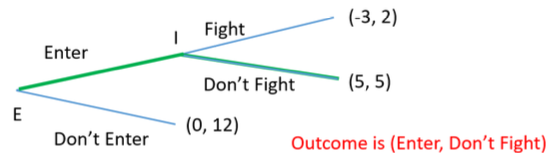
\includegraphics[width=\columnwidth]{tree1.png}

\begin{wrapfigure}{r}{0.5\columnwidth}
    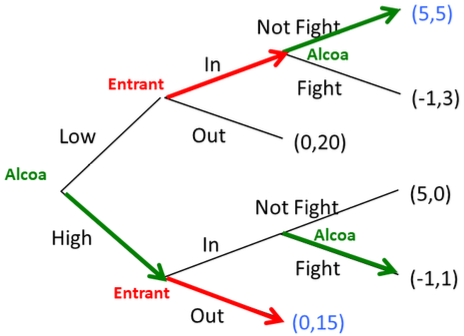
\includegraphics[width=0.5\columnwidth]{tree2.png}
\end{wrapfigure}
\Blue{Strategic Pre-commitment} a player makes a choice that commits them to a certain strategy in the future \Hint{to get rivals to respond in desirable ways}. \Green{Eg.} a firm that builds a large factory to signal that it will produce a large quantity in the future.

\begin{itemize}
    \item pre-committing aggressive actions: when rivals'll respond by being less aggressive (\eg capacity)
    \item vice versa (\eg price)
\end{itemize}

\Green{Practice Problem: simultaneous vs A pays to move first}
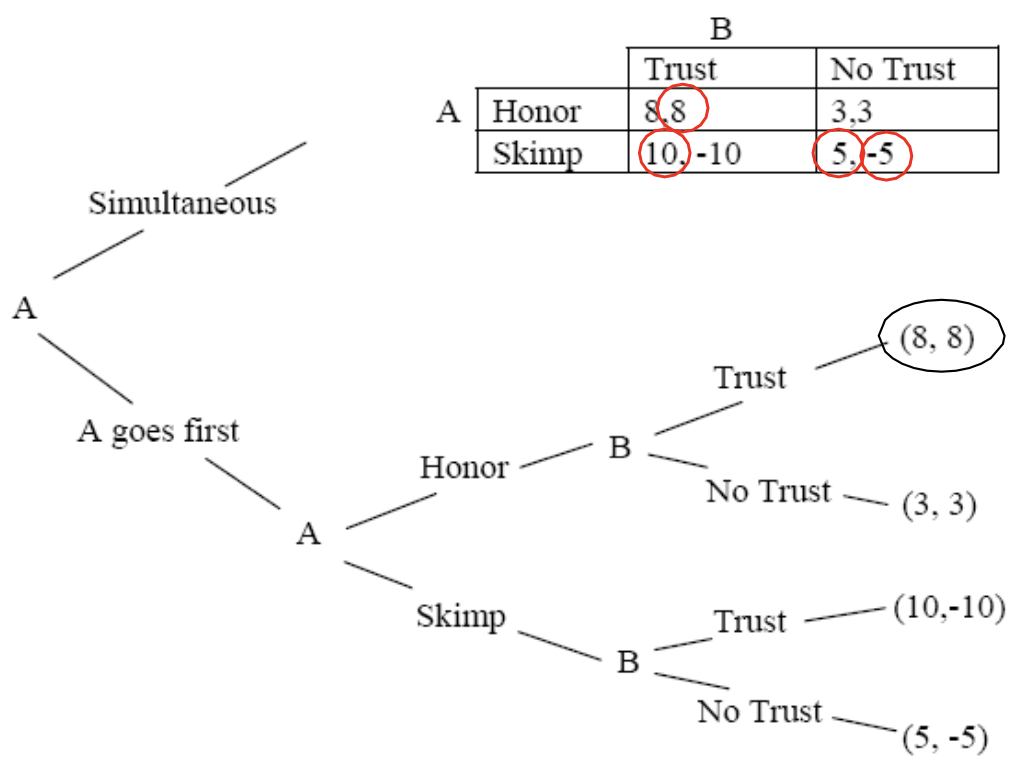
\includegraphics[width=\columnwidth]{game_theory_practice_problem.png}
\begin{itemize}
    \item Simultaneous: A's dominant strategy is ``Skimp'' (\ie save money). N.E. is (Skimp, No Trust).
    \item A would pay up to $8-5=3$ to go first reaching N.E.: (A: Honor, then B: Trust); 8 is the first-mover payoff; 5 is the simultaneous payoff.
\end{itemize}

\end{multicols}
\end{document}